%!TEX root=main.tex
\section{Results}
\label{sec:bbmm_results}

We evaluate the BBMM framework, demonstrating:
\begin{enumerate}
	\item the BBMM inference engine provides a substantial speed benefit over Cholesky based inference and standard MVM-based CG inference, especially for GPU computing;
	\item BBMM achieves comparable or better final test error compared to Cholesky inference, even with no kernel approximations; and
	\item preconditioning provides a substantial improvement in the efficiency of our approach.
\end{enumerate}

\paragraph{Baseline methods.}
We test BBMM on three types of GPs:
1. {\bf Exact} GP models,
2. {\bf SGPR} inducing point models \cite{titsias2009variational,hensman2013gaussian},
and 3. {\bf KISS-GP} models with Toeplitz $\bK_{\bZ\bZ}$ and deep kernels \cite{wilson2015kernel,wilson2016deep}.
For Exact and SGPR, we compare BBMM against Cholesky-based inference engines implemented in GPFlow \cite{matthews2017gpflow}.
GPFlow is presently the fastest implementation of these models with a Cholesky inference engine.
Since KISS-GP is not intended for Cholesky inference, we compare BBMM to the inference procedure of \citet{dong2017scalable}, implemented in our GPyTorch package.
This procedure differers from BBMM in that it computes $\trainK^{-1} \by$ without a preconditioner and computes $\log \vert \trainK \vert$ and its derivative with the Lanczos algorithm.

\paragraph{Datasets.}
We test Exact GPs on five datasets from the UCI dataset repository \cite{asuncion2007uci} with up to 3500 training examples: Skillcraft, Gas, Airfoil, Autompg, and Wine.
We test SGPR on larger datasets ($N$ up to 50000): KEGG, Protein, Elevators, Kin40k, and PoleTele.
For KISS-GP we test five large UCI datasets ($N$ up to 515000): Song, Buzz, Protein, Kin40k, and KEGG.

\paragraph{Experiment details.} All methods use the same optimizer (Adam) with identical hyperparameters.
In BBMM experiments we use rank $R\!=\!5$ pivoted Cholesky preconditioners unless otherwise stated.
We use a maximum of $J\!=\!20$ iterations of CG for each solve, and
we use $T\!=\!10$ probe vectors filled with Rademacher random variables to estimate the log determinant and trace terms.
SGPR models use $M\!=\!300$ inducing points.
KISS-GP models use $M\!=\!10,\!000$ inducing points and the deep kernels described in \cite{wilson2016deep}.
BBMM training is implemented in our GPyTorch package.
All speed experiments are run on an Intel Xeon E5-2650 CPU and an NVIDIA Titan XP GPU.

\begin{figure}[t]
  \centering
  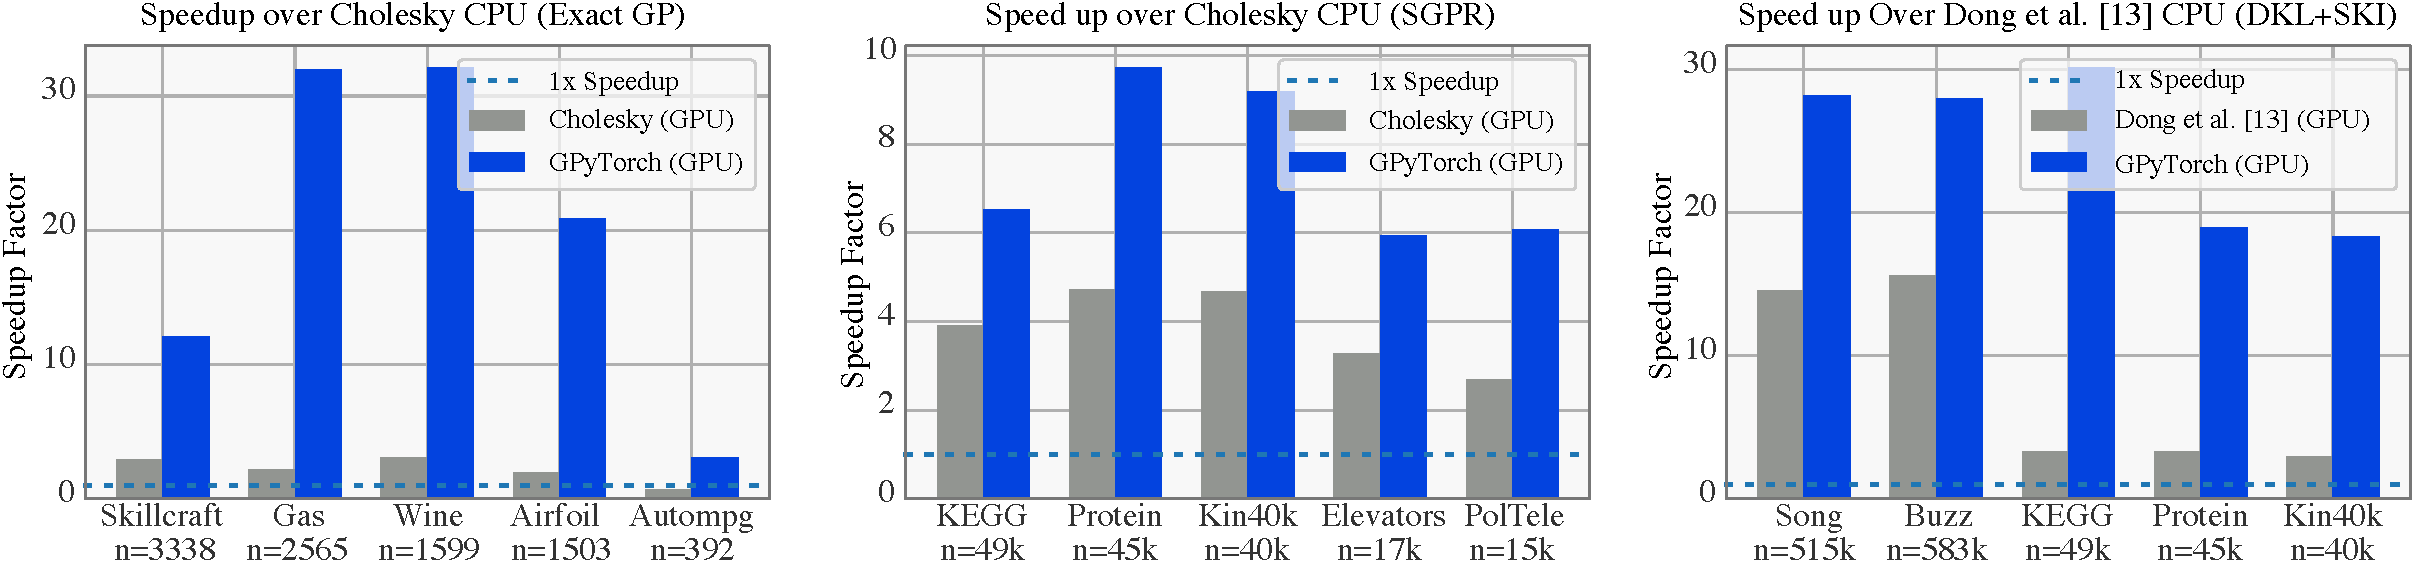
\includegraphics[width=\textwidth]{figures/sparse_gp_results}
  \caption[Speedup of GPU-accelerated GP training.]{
    Speedup of GPU-accelerated GP training.
    BBMM is in blue; competing GPU methods are in gray.
    {\bf Left:} Exact GPs speedup over CPU Cholesky-based training.
    {\bf Middle:} SGPR \cite{titsias2009variational,hensman2013gaussian} speedup over CPU Cholesky-based training.
    {\bf Right:} KISS-GP+DKL \cite{wilson2015kernel,wilson2016deep} speedup over CPU training of \citet{dong2017scalable}.
    \label{fig:timing_results}
  }
\end{figure}
%
\begin{figure}[t]
  \centering
  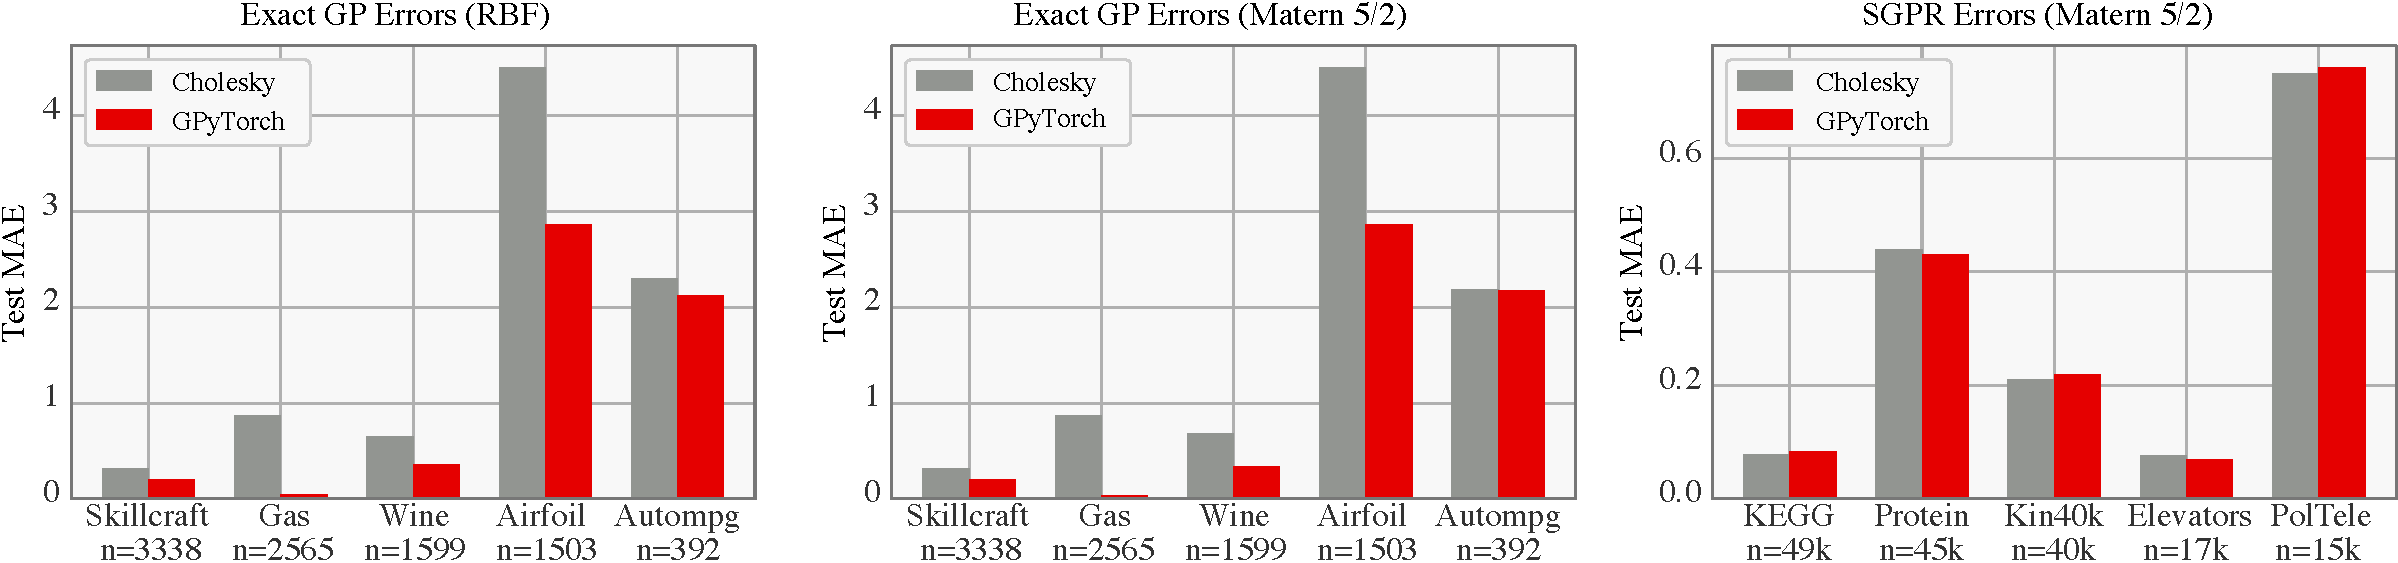
\includegraphics[width=\textwidth]{figures/exact_gp_chol_vs_mvm}
  \caption[Predictive error comparison of mBCG versus Cholesky.]{
		Predictive error comparison of mBCG versus Cholesky (MAE of predictive mean).
		The left two plots compare errors using Exact GPs with RBF and Mat\'ern-5/2 kernels,
		and the final plot compares error using SGPR with a Mat\'ern-5/2 kernel on significantly larger datasets.
	}
  \label{fig:bbmm_error_results}
\end{figure}

\paragraph{Speed comparison.}
\cref{fig:timing_results} shows the speedup obtained by GPU-accelerated BBMM over CPU-based training methods (Cholesky for Exact/SGPR, \citet{dong2017scalable} for KISS-GP).
As would be expected, GPU-accelerated BBMM is faster than CPU-based inference.
On Exact and KISS-GP, BBMM is up to \emph{32 times faster} than CPU inference, and up to 10 times faster on SGPR.
The largest speedups occur on the biggest datasets, since smaller datasets experience larger GPU overhead.
Notably, BBMM achieves a much larger speedup than GPU accelerated Cholesky methods (Exact, SGPR), which only achieve a roughly $4\times$ speedup.
This result underscores the fact that Cholesky methods are not as well suited for GPU acceleration.
Additionally, BBMM performs better than the GPU-accelerated version of \cite{dong2017scalable} on KISS-GP.
This speedup is because BBMM is able to calculate all inference terms in parallel, while \cite{dong2017scalable} computes the terms in series.

\begin{figure}[t!]
  \begin{center}
    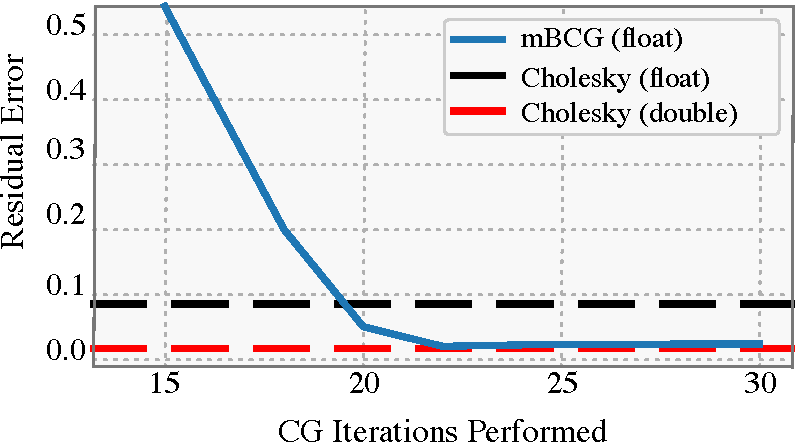
\includegraphics[width=0.48\textwidth]{figures/cg_error}
  \end{center}
  \caption{Solve error for mBCG and Cholesky. \label{fig:cg_error}}
\end{figure}

\paragraph{Predictive error comparison.}
The predictive mean, given by \cref{eqn:predictive_mean}, requires computing the solve $\trainK^{-1} \by$.
Therefore, the mBCG algorithm can be used to compute this term with preconditioning and GPU acceleration.
In \cref{fig:bbmm_error_results} we compare the mean average error (MAE) computed using mBCG verses Cholesky.\footnote{
  KISS-GP models are excluded from \cref{fig:bbmm_error_results}, as the KISS-GP predictive mean is computed using CG.
}
We demonstrate results using both the RBF kernel and a Mat\'ern-5/2 kernel.
Across all datasets, our method is at least as accurate in terms of final test MAE.
On a few datasets (e.g. Gas, Airfoil, and Wine with Exact GPs) BBMM even improves final test error.

CG has a regularizing effects which may improve methods involving the exact kernel over the Cholesky decomposition, where numerical issues resulting from extremely small eigenvalues of the kernel matrix are ignored.
For example, Cholesky methods frequently add noise (or ``jitter'') to the diagonal of the kernel matrix for numerical stability.
It is possible to reduce the numerical instabilities with double precision (see \cref{fig:cg_error}); however, this requires an increased amount of computation.
BBMM on the other hand avoids adding this noise, without requiring double precision.

\begin{figure}[t]
  \centering
  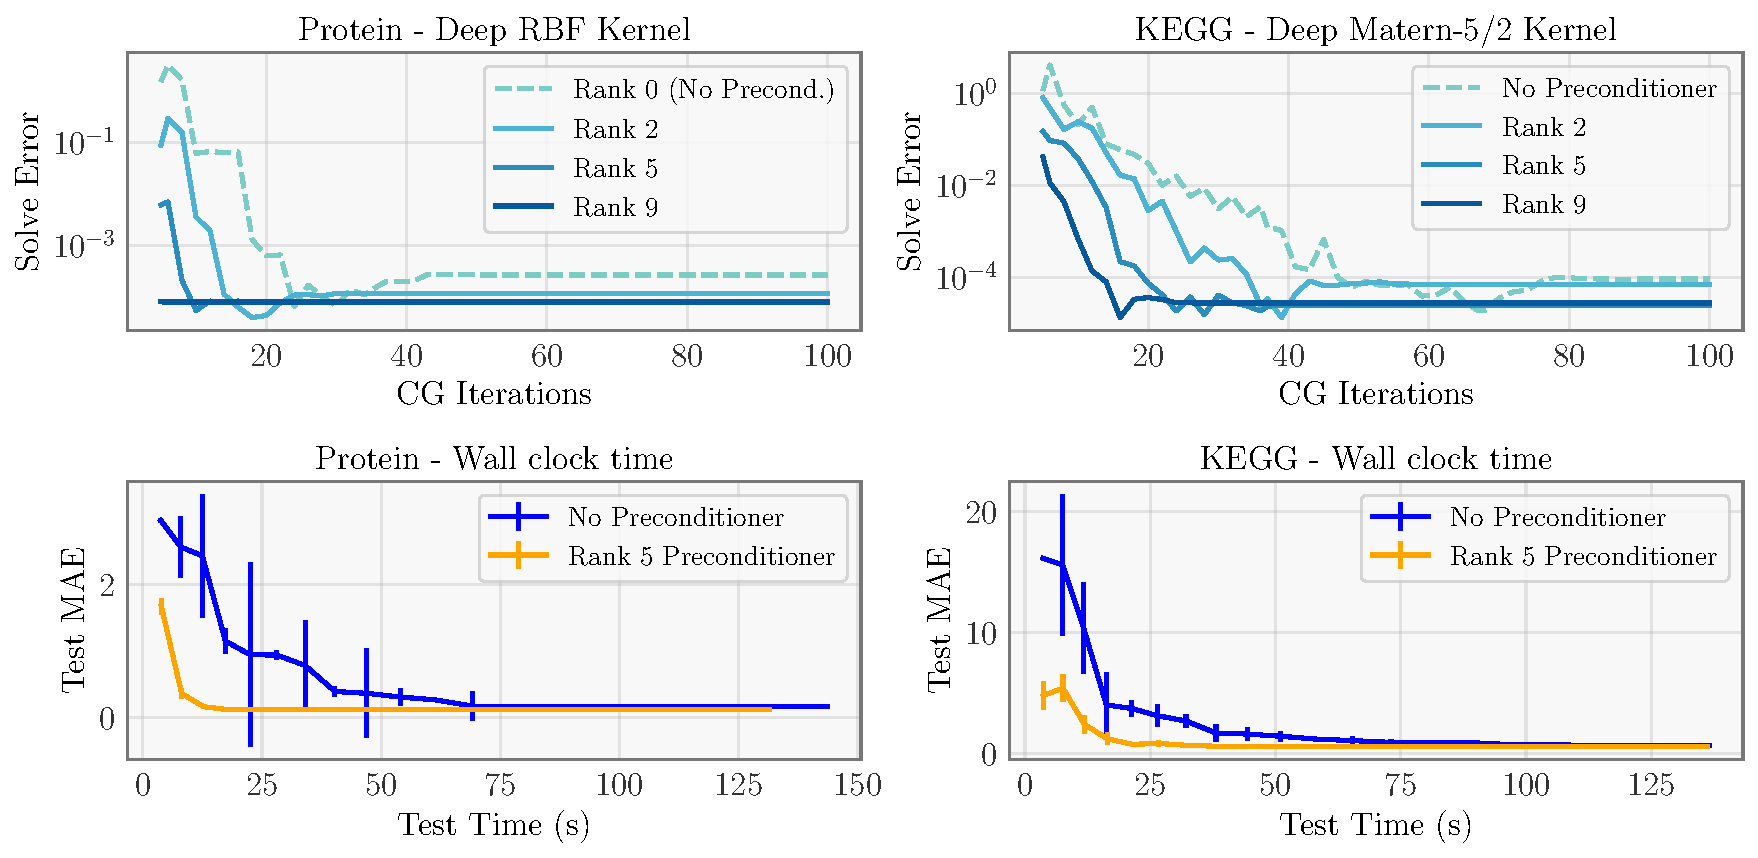
\includegraphics[width=\textwidth]{figures/precond_solves}
  \caption[Effect of partial pivoted Cholesky preconditioning on mBCG solve errors.]{
    Effect of partial pivoted Cholesky preconditioning on solve errors.
		{\bf Top:} mBCG residual $\Vert \trainK \bc - \by \Vert / \Vert \by \Vert$ verses number of mBCG iterations.
		{\bf Bottom:} Test set MAE (using \cref{eqn:predictive_mean}) verses mBCG wall-clock time.
		Solves are computed using no preconditioner, rank $R=2$, $R=5$, and $R=9$ pivoted Cholesky preconditioners using deep RBF and deep Mat\'ern kernels.
		On the 2 datasets tested (Protein and KEGG), preconditioning accelerates convergence.
  }
  \label{fig:precond_results}
\end{figure}

\paragraph{Preconditioning.}
To demonstrate the effectiveness of preconditioning at accelerating the convergence of conjugate gradients,
we train deep RBF and deep Mat\'ern-5/2 kernels on two datasets (Protein and KEGG) and evaluate the solve error of using mBCG to compute $\bc = \trainK^{-1}\by$.
We measure the relative residual $\Vert \trainK\bc - \by \Vert / \Vert \by \Vert$ as a function of the number of mBCG iterations performed.
We compare using no preconditioner, as well as rank $R=2$, $R=5$, and $R=9$ partial pivoted Cholesky preconditioners.
The results are in the top of \cref{fig:precond_results}.
As expected based on our theoretical intuitions for this preconditioner, increasing the rank of the preconditioner substantially reduces the number of mBCG iterations required to achieve convergence.

In the bottom of \cref{fig:precond_results}, we confirm that these more accurate solves indeed have an effect on the final test MAE (when using mBCG to compute the predictive mean).
We plot, as a function of the total wallclock time required to compute predictions, the test MAE resulting from using no preconditioner and from using a rank 5 preconditioner.
The wallclock time is varied by changing the number of CG iterations used to compute the predictive mean.
We observe that, because such a low rank preconditioner is sufficient, using preconditioning results in significantly more accurate solves while having virtually no impact on the running time of each CG iteration.
Consequentially, we recommend always using the pivoted Cholesky preconditioner with BBMM since it has virtually no wall-clock overhead and rapidly accelerates convergence.
